\documentclass[a4paper,12pt]{report}
\usepackage[utf8]{inputenc}
\usepackage[spanish]{babel}
\usepackage{graphicx}
\usepackage{geometry}
\usepackage{setspace}
\usepackage{titlesec}
\usepackage{cite}
\usepackage{url}
\usepackage{verbatim}
\usepackage{amsmath}
\usepackage{float}
\usepackage{caption}
\usepackage{subcaption}

% Configuración de la página
\geometry{top=2.5cm, bottom=2.5cm, left=3cm, right=3cm}

% Espaciado entre líneas
\setstretch{1.5}

% Formato de títulos
\titleformat{\chapter}{\normalfont\huge\bfseries}{\thechapter.}{20pt}{\huge}
\titleformat{\section}{\normalfont\Large\bfseries}{\thesection.}{1em}{}
\titleformat{\subsection}{\normalfont\large\bfseries}{\thesubsection.}{1em}{}

% Título, autor y fecha
\title{Algorítmos de Sincronización}
\author{Sebastián Arias, Christopher Bazurto, Stephen Drouet, Josué Merino}
\date{\today}

\begin{document}

% Portada
\begin{titlepage}
 \centering
    
\includegraphics[width=0.5\linewidth]{images/ESPE2.png}\\[1.0 cm]
    \textsc{\Large UNIVERSIDAD DE LAS FUERZAS ARMADAS ESPE}\\[2 cm]
	\textsc{\Large Aplicaciones Distribuidas}\\[0.5 cm]
	\textsc{\large Departamento de Ciencias de la Computación}\\[0.5 cm]
	\rule{\linewidth}{0.2 mm} \\[0.4 cm]
	{ \huge \bfseries Algorítmos de Sincronización}\\
	\rule{\linewidth}{0.2 mm} \\[1.5 cm]
	
    \begin{flushleft} \large
        \emph{Estudiantes:}\\
        Sebastián Arias, Christopher Bazurto, Stephen Drouet, Josué Merino
    \end{flushleft}

    \begin{flushleft} \large
        \emph{Docente:}\\
        Ing. Darío Morales\\
    \end{flushleft}
    
    \vfill
    \date{\today}
    
\end{titlepage}

\tableofcontents
\listoffigures
\newpage
\chapter{Objetivos}

\section{Objetivo Principal}
Implementar la sincronización de relojes en un sistema distribuido mediante tres métodos: NTP, el algoritmo de Cristian y el algoritmo de Berkeley, con el fin de lograr una sincronización precisa entre múltiples nodos de un sistema. 
\section{Objetivos Específicos}
\begin{itemize}
    \item Implementar el cliente NTP: Desarrollar una aplicación que consulte un servidor de tiempo (como "time.google.com") y ajuste el reloj local en base a la hora proporcionada por dicho servidor.
    \item Implementar el Algoritmo de Cristian: Crear una aplicación cliente-servidor donde el cliente consulte a un servidor de tiempo para estimar la hora exacta, teniendo en cuenta la latencia de la red.
    \item Simular el Algoritmo de Berkeley: Desarrollar una simulación en la que varios nodos (hilos o instancias) ajusten sus relojes mediante la colaboración para llegar a un tiempo promedio.
    \item Generar el Informe: Documentar el proceso de implementación y funcionamiento de cada algoritmo, explicando las fases de sincronización y los resultados obtenidos.
    \item Proveer Evidencias: Incluir capturas de pantalla o videos demostrando los resultados de la sincronización de los relojes.
\end{itemize}

\chapter{Desarrollo}
\section{NTP}
Es un protocolo de Internet para sincronizar los relojes de los sistemas informáticos a través del enrutamiento de paquetes en redes con latencia variable. NTP utiliza UDP como su capa de transporte, usando el puerto 123. Está diseñado para resistir los efectos de la latencia variable. \cite{ntp}

\subsection{Código}
Al crear el proyecto se agregan las dependencias en pom.xml
\begin{verbatim}
<dependency>
    <groupId>commons-net</groupId>
    <artifactId>commons-net</artifactId>
    <version>3.7</version>
</dependency>
\end{verbatim}

Se crea el archivo NTPClient:
\begin{verbatim}
import org.apache.commons.net.ntp.NTPUDPClient;
import org.apache.commons.net.ntp.TimeInfo;
import java.net.InetAddress;
import java.util.Date;

class NTPClient {
    public static void main(String[] args) {
        try {
            String ntpServer = "time.google.com";
            NTPUDPClient client = new NTPUDPClient();
            client.setDefaultTimeout(10000); 
            InetAddress inetAddress = InetAddress.getByName(ntpServer);
            TimeInfo timeInfo = client.getTime(inetAddress);
            long returnTime = timeInfo.getMessage().getTransmitTimeStamp().getTime();
            Date currentDate = new Date(returnTime);
            System.out.println("Hora sincronizada con el servidor NTP: "
            + currentDate);
        } catch (Exception e) {
            System.err.println("Error al sincronizar con el servidor NTP: " 
            + e.getMessage());
        }
    }
}
\end{verbatim}
\subsection{Explicación}


\begin{itemize}
    \item Librería NTP: Se usa la librería commons-net para interactuar con el servidor NTP.
    \item NTPUDPClient: Es la clase que proporciona la funcionalidad para consultar un servidor NTP a través de UDP.
    \item TimeInfo: Representa la respuesta del servidor, que incluye la hora en el servidor.
    \item Conexión al servidor: El cliente se conecta a time.google.com y consulta el tiempo.
    \item Tiempo: La respuesta contiene el tiempo de transmisión, que se convierte en un objeto Date para mostrar la hora.
    \item Manejo de excepciones: Si ocurre algún error, se captura y muestra un mensaje.
\end{itemize}

\subsection{Capturas y Evidencias}
\begin{figure} [H]
    \centering
    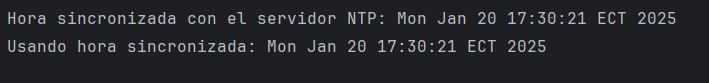
\includegraphics[width=1\linewidth]{images/ntp.png}
    \caption{NTP}
    \label{fig:enter-label}
\end{figure}

\section{Cristian’s Algorithm}
Es un método, dentro de la computación distribuida, para la sincronización de relojes. Cristian describe el método como probabilístico debido a que se consigue sincronización solo si el tiempo de respuesta es suficientemente corto comparado con la precisión requerida. Consiste en un servidor conectado a una fuente de UTC y unos clientes que se sincronizan con dicho servidor. \cite{cristian}
\subsection{¿Cómo funciona el Algoritmo de Cristian?}
El algoritmo de Cristian se basa en los siguientes pasos:
\begin{enumerate}
    \item El cliente envía una solicitud de tiempo al servidor: El cliente le pide al servidor su hora actual.
    \item El servidor responde con su hora: El servidor devuelve su hora actual (típicamente utilizando NTP o un mecanismo similar).
    \item El cliente recibe la hora del servidor: El cliente recibe la respuesta del servidor junto con el tiempo que ha pasado desde que hizo la solicitud.
    \item El cliente estima la hora del servidor: Usando la hora que le devolvió el servidor y la latencia de la red, el cliente calcula una estimación de la hora exacta del servidor.
\end{enumerate}

\begin{itemize}
  \item \( T_1 \) = Tiempo de solicitud enviado por el cliente
  \item \( T_2 \) = Tiempo de respuesta recibido por el servidor
  \item \( T_3 \) = Tiempo de respuesta recibido por el cliente
  \item \( T_4 \) = Tiempo de solicitud recibido por el servidor
\end{itemize}

La estimación de la hora exacta del servidor es:

\[
T_s = T_2 + \frac{T_3 - T_1}{2}
\]


\subsection{Código}
Se crea el servidor:
\begin{verbatim}
package com.espe.cristian;

import java.io.*;
import java.net.*;
import java.util.Date;

class TimeServer {
    public static void main(String[] args) {
        try {
            // Puerto en el que el servidor escuchará
            int port = 12345;
            DatagramSocket socket = new DatagramSocket(port);
            System.out.println("Servidor esperando conexiones...");

            // Bucle para recibir solicitudes de los clientes
            while (true) {
                byte[] receiveData = new byte[1024];

                // Recibir la solicitud del cliente
                DatagramPacket receivePacket = 
                new DatagramPacket(receiveData, receiveData.length);
                socket.receive(receivePacket);

                // Obtener la hora actual
                long serverTime = System.currentTimeMillis();
                String serverTimeString = Long.toString(serverTime);

                // Enviar la respuesta con la hora del servidor
                InetAddress clientAddress = receivePacket.getAddress();
                int clientPort = receivePacket.getPort();
                DatagramPacket sendPacket = 
                new DatagramPacket(serverTimeString.getBytes(),
                serverTimeString.length(), clientAddress, clientPort);
                socket.send(sendPacket);
                System.out.println("Hora enviada al cliente: " + serverTime);
            }
        } catch (Exception e) {
            e.printStackTrace();
        }
    }
}
\end{verbatim}
Paso siguiente se crea el cliente:
\begin{verbatim}
package com.espe.cristian;

import java.net.*;
import java.util.Date;

class TimeClient {
    public static void main(String[] args) {
        try {
            // Dirección y puerto del servidor
            String serverAddress = "localhost";
            int serverPort = 12345;

            // Crear el socket
            DatagramSocket socket = new DatagramSocket();

            // Establecer el tiempo de solicitud (T1)
            long T1 = System.currentTimeMillis();
            byte[] sendData = new byte[1024];
            String requestMessage = "Hora solicitada";
            sendData = requestMessage.getBytes();

            // Enviar la solicitud al servidor
            InetAddress serverInetAddress = InetAddress.getByName(serverAddress);
            DatagramPacket sendPacket = 
            new DatagramPacket(sendData, sendData.length, 
            serverInetAddress, serverPort);
            socket.send(sendPacket);
            System.out.println("Solicitud enviada al servidor...");

            // Recibir la respuesta del servidor
            byte[] receiveData = new byte[1024];
            DatagramPacket receivePacket = 
            new DatagramPacket(receiveData, receiveData.length);
            socket.receive(receivePacket);
            long T3 = System.currentTimeMillis(); 
            // Hora cuando se recibe la respuesta

            // Obtener la hora del servidor (T2)
            String serverTimeString = 
            new String(receivePacket.getData(), 0,
            receivePacket.getLength());
            long T2 = Long.parseLong(serverTimeString);

            // Calcular la hora estimada del servidor (T_s)
            long T_s = T2 + ((T3 - T1) / 2);

            // Mostrar los resultados
            System.out.println("Hora solicitada por el cliente (T1): "
            + new Date(T1));
            System.out.println("Hora recibida del servidor (T2): "
            + new Date(T2));
            System.out.println("Hora recibida por el cliente (T3): "
            + new Date(T3));
            System.out.println("Hora estimada del servidor (T_s): "
            + new Date(T_s));

            socket.close();
        } catch (Exception e) {
            e.printStackTrace();
        }
    }
}

\end{verbatim}
\subsection{Explicación}
El servidor escucha en el puerto 12345.
Recibe la solicitud del cliente y obtiene la hora actual del sistema.
Envía esa hora de vuelta al cliente.
El cliente envía una solicitud al servidor.
Mide el tiempo T1 (cuando se envía la solicitud) y T3 (cuando se recibe la respuesta).
Usa la hora T2 proporcionada por el servidor para estimar la hora exacta del servidor utilizando la fórmula: \[
T_s = T_2 + \frac{T_3 - T_1}{2}
\]
\subsection{Capturas y Evidencias}
Se ejecuta primero el servidor:
\begin{figure} [H]
    \centering
    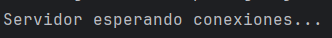
\includegraphics[width=1\linewidth]{images/server1.png}
    \caption{Ejecución del Servidor}
    \label{fig:enter-label}
\end{figure}
Después se ejecuta el cliente:
\begin{figure} [H]
    \centering
    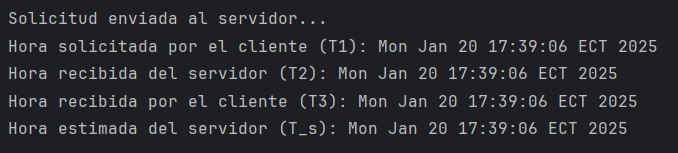
\includegraphics[width=1\linewidth]{images/client1.png}
    \caption{Ejecución del Cliente}
    \label{fig:enter-label}
\end{figure}
El servidor muestra la hora envíada al cliente:
\begin{figure} [H]
    \centering
    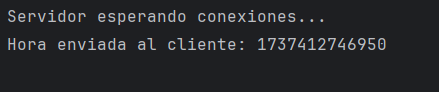
\includegraphics[width=1\linewidth]{images/servidor2.png}
    \caption{Hora enviada al cliente desde el servidor}
    \label{fig:enter-label}
\end{figure}
1737412746950 es el número de milisegundos desde el 1 de enero de 1970 a la medianoche (hora UTC). En términos prácticos, esto es el equivalente a una fecha y hora específica.

\section{Algoritmo de Berkeley}
Se trata de un algoritmo de sincronización de relojes diseñado por Gusella y Zatti en 1989. Dicho algoritmo se creó para entornos en los cuales no se tienen receptores de tiempo UTC, de forma que, gracias a este algoritmo se pueden mantener los relojes del entorno sincronizados con la misma hora. Este algoritmo sincroniza procesos en un sistema distribuido y garantiza que estos mismos se ejecuten de manera cronológica y secuencial (respetando el orden de los eventos en el sistema). Este algoritmo se categoriza como un algoritmo de sincronización de relojes físicos e internos. La base de todos estos tipos de algoritmos es la comunicación del tiempo de reloj de cada nodo. Cada uno calcula alguna función de tipo promedio o la mediana de todos los valores, si la diferencia con su reloj actual es mayor que la desviación máxima permitida se actualiza el reloj con el nuevo valor. Posteriormente el algoritmo se ejecutará de nuevo hasta lograr una convergencia de todos los nodos. \cite{berkeley}


\subsection{Código}
Se crea un BerkeleyServer.java para manejar la lógica del servidor, que recibe los tiempos de los nodos, calcula el tiempo promedio y ajusta los relojes de los nodos.
\begin{verbatim}
package com.espe.berkeley;

import java.text.SimpleDateFormat;
import java.util.*;

public class BerkeleyServer {
    private static final int NUM_NODES = 5;  // Número de nodos en el sistema
    private List<ClockNode> nodes;  // Lista de nodos
    private long averageTime;  // Tiempo promedio calculado

    public BerkeleyServer() {
        nodes = new ArrayList<>();
        // Crear y añadir nodos al servidor
        for (int i = 1; i <= NUM_NODES; i++) {
            nodes.add(new ClockNode(i, this));
        }
    }

    // Método para recibir los tiempos de los nodos y calcular el promedio
    public void receiveTimesAndCalculateAverage() {
        long total = 0;
        for (ClockNode node : nodes) {
            total += node.getLocalTime();
            System.out.println("Servidor recibe tiempo del nodo " 
            + node.getNodeId() + ": " 
            + formatTime(node.getLocalTime()));
        }

        averageTime = total / nodes.size();
        System.out.println("Servidor calcula el tiempo promedio: " 
        + formatTime(averageTime));
    }

    // Método para enviar el tiempo promedio a los nodos
    public void adjustNodeTimes() {
        for (ClockNode node : nodes) {
            node.adjustTime(averageTime);
        }
    }

    // Formato para mostrar el tiempo legible
    private String formatTime(long timeInMillis) {
        SimpleDateFormat sdf = new SimpleDateFormat("yyyy-MM-dd HH:mm:ss.SSS");
        Date date = new Date(timeInMillis);
        return sdf.format(date);
    }

    // Método principal para ejecutar la simulación
    public static void main(String[] args) {
        BerkeleyServer server = new BerkeleyServer();

        // Recibir tiempos de los nodos y calcular el promedio
        server.receiveTimesAndCalculateAverage();

        // Ajustar los tiempos de los nodos según el tiempo promedio
        server.adjustNodeTimes();
    }
}
\end{verbatim}
Se crea una clase ClockNode.java que representa a cada nodo en el sistema con su propio reloj. Cada nodo tiene un desfase aleatorio simulado para mostrar cómo los relojes pueden desincronizarse antes de que el servidor los sincronice.
\begin{verbatim}
package com.espe.berkeley;

import java.text.SimpleDateFormat;
import java.util.*;

public class ClockNode {
    private int nodeId;
    private long localTime;  // Tiempo local del nodo
    private BerkeleyServer server;  // Referencia al servidor

    public ClockNode(int nodeId, BerkeleyServer server) {
        this.nodeId = nodeId;
        this.server = server;

        // Simular un desfase aleatorio de -500 a 500 ms
        Random random = new Random();
        this.localTime = System.currentTimeMillis() + random.nextInt(1000) - 500;
    }

    // Obtener el tiempo local del nodo
    public long getLocalTime() {
        return localTime;
    }

    // Obtener el ID del nodo
    public int getNodeId() {
        return nodeId;
    }

    // Ajustar el reloj del nodo según el tiempo promedio
    public void adjustTime(long averageTime) {
        localTime = averageTime;
        System.out.println("Nodo " + nodeId + " ajusta su tiempo a: " 
        + formatTime(localTime));
    }

    // Formato para mostrar el tiempo legible
    private String formatTime(long timeInMillis) {
        SimpleDateFormat sdf = new SimpleDateFormat("yyyy-MM-dd HH:mm:ss.SSS");
        Date date = new Date(timeInMillis);
        return sdf.format(date);
    }
}
\end{verbatim}
Main.java: Este archivo contiene el método main donde se crea el servidor y se ejecuta el proceso de sincronización de los nodos.
\begin{verbatim}
package com.espe.berkeley;

public class Main {
    public static void main(String[] args) {
        BerkeleyServer server = new BerkeleyServer();

        // Recibir tiempos de los nodos y calcular el promedio
        server.receiveTimesAndCalculateAverage();

        // Ajustar los tiempos de los nodos según el tiempo promedio
        server.adjustNodeTimes();
    }
}
\end{verbatim}
\subsection{Explicación}
\begin{itemize}
    \item Simula un sistema con 5 nodos.
    \item El servidor recibe los tiempos de los nodos, calcula el tiempo promedio y luego ajusta los relojes de los nodos a ese tiempo promedio.
    \item Los tiempos de los nodos son inicialmente desincronizados debido a un desfase aleatorio.
\end{itemize}

\subsection{Capturas y Evidencias}
\begin{figure}
    \centering
    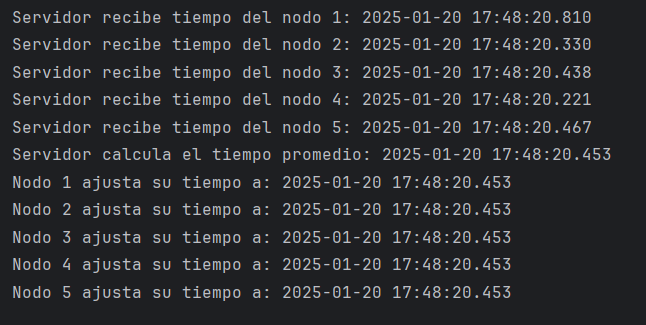
\includegraphics[width=1\linewidth]{images/berkeley.png}
    \caption{Algorítmo de Berkeley}
    \label{fig:enter-label}
\end{figure}

\section{Enlaces} 
Repositorio: \url{https://github.com/ejmerino/algoritmos-de-sincronizacion}

\chapter{Conclusiones}
\begin{itemize}
    \item La implementación del cliente NTP demostró ser efectiva para sincronizar el reloj local con precisión al consultar servidores de tiempo confiables, como "time.google.com". El protocolo NTP es robusto y se adapta a diferentes latencias de red sin comprometer la precisión.

    \item Al considerar la latencia de red, fue exitoso para estimar un tiempo preciso, aunque la precisión depende de la estabilidad y la latencia de la conexión. Este método permite obtener una sincronización más exacta que simplemente consultar un servidor de tiempo sin considerar la red.

    \item  La simulación del algoritmo de Berkeley en un sistema distribuido con varios nodos fue exitosa. El ajuste de los relojes de los nodos para alcanzar un promedio proporcionó un buen resultado en términos de precisión en sistemas distribuidos. Este algoritmo demuestra la importancia de la colaboración entre nodos para mantener la sincronización a través de redes no confiables.

    \item Todos los métodos implementados demostraron que, a pesar de las variaciones en la latencia de red o el número de nodos, es posible lograr una sincronización precisa de relojes en sistemas distribuidos, lo cual es fundamental en aplicaciones que requieren alta precisión temporal.

    \item Las capturas de pantalla y videos mostraron claramente la sincronización exitosa de los relojes entre el cliente y los servidores, y entre los nodos en el caso del algoritmo de Berkeley, lo que valida la correcta implementación de los algoritmos.

\end{itemize}

\begin{thebibliography}{99}
\bibitem{ntp} Tecnozero. (2023, 25 abril). Servidor NTP o Servidor de hora. Tecnozero Soluciones Informaticas. \url{https://www.tecnozero.com/servidor/ntp/}
\bibitem{cristian} colaboradores de Wikipedia. (2023, 31 enero). Algoritmo de Cristian. Wikipedia, la Enciclopedia Libre. \url{https://es.wikipedia.org/wiki/Algoritmo_de_Cristian#:~:text=El%20algoritmo%20de%20Cristian%20(1989,comparado%20con%20la%20precisi%C3%B3n%20requerida. }
\bibitem{berkeley} colaboradores de Wikipedia. (2022, 2 julio). Algoritmo de Berkeley. Wikipedia, la Enciclopedia Libre. \url{https://es.wikipedia.org/wiki/Algoritmo_de_Berkeley}

\end{thebibliography}

\end{document}